% =====================================================================
%  DSP391m · Group 5 — Data Tasks (English) — CCNU-style Beamer deck
%  Reproduces the look of task/CCNU_presentation_Beamer.pdf:
%  Madrid (sans), crimson frame titles on a light bar, dark-red footer,
%  navy TOC balls + block headers, booktabs red-header tables, Outline
%  frames between sections. Compile with Tectonic (XeTeX).
% =====================================================================
\documentclass[aspectratio=169,10pt]{beamer}

\usetheme{Madrid}
\usecolortheme{beaver}
\setbeamertemplate{navigation symbols}{}
\setbeamertemplate{caption}{\insertcaption}

\usepackage{iftex}
\ifPDFTeX
  \usepackage[T1]{fontenc}
  \usepackage[utf8]{inputenc}
  \usepackage{lmodern}
\else
  \usepackage{fontspec}              % XeTeX/Tectonic — keep sans (Latin Modern Sans)
\fi
\usepackage{booktabs}
\usepackage{array}
\usepackage{tabularx}
\usepackage{colortbl}
\usepackage{tikz}
\usepackage{pgfplots}
\pgfplotsset{compat=1.18}
\usetikzlibrary{arrows.meta,positioning}
\usepackage{graphicx}
\graphicspath{{../figures/}{figures/}{./}}

% ---- CCNU palette: crimson primary + navy secondary ----
\definecolor{ccnured}{HTML}{C00000}
\definecolor{ccnudark}{HTML}{7A0E12}
\definecolor{ccnunavy}{HTML}{31318A}
\definecolor{rowtint}{HTML}{F4ECEC}

\setbeamercolor{frametitle}{fg=ccnured,bg=black!6}
\setbeamercolor{title}{fg=ccnured}
\setbeamercolor{structure}{fg=ccnured}
\setbeamercolor{section number projected}{bg=ccnunavy,fg=white}
\setbeamercolor{item projected}{bg=ccnunavy,fg=white}
\setbeamercolor{itemize item}{fg=ccnunavy}
\setbeamercolor{itemize subitem}{fg=ccnured}
\setbeamercolor{block title}{bg=ccnunavy,fg=white}
\setbeamercolor{block body}{bg=ccnunavy!8}
\setbeamerfont{frametitle}{series=\bfseries}
\setbeamertemplate{section in toc}[ball]
\setbeamertemplate{blocks}[rounded][shadow=true]

% ---- helpers ----
\newcolumntype{Y}{>{\raggedright\arraybackslash}X}
\newcommand{\hc}[1]{{\bfseries\color{white}#1}}
\newcommand{\tcode}[1]{{\ttfamily #1}}
\newcommand{\takeaway}[1]{\vspace{2pt}\par{\footnotesize\itshape #1}}

\AtBeginSection[]{%
  \begin{frame}{Outline}
    \tableofcontents[currentsection]
  \end{frame}}

% ---- meta ----
\title[Data Tasks]{Data Tasks: Collection \& Preprocessing}
\subtitle{EduGuard: AI-Powered Early Warning and Actionable Recourse System for Students}
\author[Group 5 -- DSP391m]{Group 5 -- DSP391m}
\institute[FPT University]{FPT University}
\date[DSP391m 2026]{Data Science Capstone (DSP391m) \textbullet{} Report 2}

\begin{document}

\begin{frame}[plain]\titlepage\end{frame}

\begin{frame}{Table of Contents}\tableofcontents\end{frame}

% =====================================================================
\section{Required Data for the Study}
% =====================================================================
\begin{frame}{Data Requirements}
  {\footnotesize
  \setlength{\tabcolsep}{5pt}\renewcommand{\arraystretch}{1.3}
  \begin{tabularx}{\textwidth}{@{}>{\raggedright\arraybackslash}p{3.2cm} Y >{\raggedright\arraybackslash}p{4.0cm}@{}}
    \toprule
    \rowcolor{ccnured}\hc{Requirement} & \hc{Why it is required} & \hc{OULAD source}\\
    \midrule
    Binary at-risk label & Prediction target — used by all three RQs & \tcode{studentInfo.final\_result}\\
    \rowcolor{rowtint}
    Time-stamped engagement & Time-aware checkpoint features (RQ1/RQ2) & \tcode{studentVle} ($\sim$10.6M), \tcode{vle}\\
    Academic performance & Early score signals up to each checkpoint & \tcode{studentAssessment}, \tcode{assessments}\\
    \rowcolor{rowtint}
    Demographic context & Baseline covariates + fairness analysis & \tcode{studentInfo}, \tcode{studentRegistration}\\
    Course timeline & Convert event dates to progress \% & \tcode{courses.module\_presentation\_length}\\
    \bottomrule
  \end{tabularx}}
  \takeaway{Three feature groups on the key \tcode{(id\_student, code\_module, code\_presentation)}: Demographic \textbullet{} Engagement (VLE) \textbullet{} Performance (assessments).}
\end{frame}

\begin{frame}{OULAD at a Glance}
  \begin{columns}[T]
    \begin{column}{0.42\textwidth}
      \footnotesize\textbf{Scale of the dataset}
      \begin{itemize}\setlength\itemsep{0.25em}
        \item \textbf{32,593} student–module–presentation records
        \item \textbf{28,785} unique students
        \item \textbf{22} module-presentations, \textbf{7} tables
        \item \textbf{10,655,280} VLE click events
        \item $\sim$\textbf{173,912} assessment submissions
        \item Daily resolution (2013–2014)
      \end{itemize}
      \takeaway{The Open University (UK); \textbf{CC-BY 4.0}, anonymised at source.}
    \end{column}
    \begin{column}{0.58\textwidth}
      {\scriptsize
      \setlength{\tabcolsep}{4pt}\renewcommand{\arraystretch}{1.25}
      \begin{tabularx}{\textwidth}{@{}>{\ttfamily}l Y c@{}}
        \toprule
        \rowcolor{ccnured}\hc{Table} & \hc{Role} & \hc{Time?}\\
        \midrule
        studentInfo & Outcome label + demographics & no\\
        \rowcolor{rowtint}studentRegistration & Registration / withdrawal dates & part\\
        studentVle & Clickstream ($\sim$10.6M rows) & \textbf{yes}\\
        \rowcolor{rowtint}vle & Maps site $\to$ activity type & no\\
        studentAssessment & Submissions + scores & \textbf{yes}\\
        \rowcolor{rowtint}assessments & Type, weight, deadline & part\\
        courses & Presentation length (days) & no\\
        \bottomrule
      \end{tabularx}}
      \takeaway{\tcode{studentVle.date} and \tcode{studentAssessment.date\_submitted} are the foundation of the time-aware design.}
    \end{column}
  \end{columns}
\end{frame}

\begin{frame}{Target Variable \& Class Balance}
  \begin{columns}[T]
    \begin{column}{0.54\textwidth}
      {\scriptsize
      \setlength{\tabcolsep}{5pt}\renewcommand{\arraystretch}{1.3}
      \begin{tabularx}{\textwidth}{@{}>{\ttfamily}l Y Y@{}}
        \toprule
        \rowcolor{ccnured}\hc{final\_result} & \hc{Group} & \hc{Label}\\
        \midrule
        Distinction & Pass & not-at-risk (0)\\
        \rowcolor{rowtint}Pass & Pass & not-at-risk (0)\\
        Fail & At-risk & \textbf{at-risk (1)}\\
        \rowcolor{rowtint}Withdrawn & At-risk & \textbf{at-risk (1)}\\
        \bottomrule
      \end{tabularx}}
      \vspace{3pt}\par\footnotesize
      \tcode{at\_risk = final\_result $\in$ \{Fail, Withdrawn\}}
      \begin{itemize}\setlength\itemsep{0.15em}
        \item Label \textbf{fixed} across all six checkpoints.
        \item Imbalance is \textbf{mild} ($\approx$52.8\% at-risk).
        \item Metrics: \textbf{PR-AUC} + \textbf{recall} on the at-risk class.
      \end{itemize}
    \end{column}
    \begin{column}{0.46\textwidth}
      \centering
      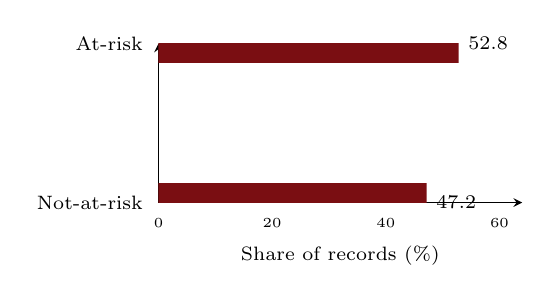
\begin{tikzpicture}
        \begin{axis}[width=6.2cm,height=3.6cm,xbar,xmin=0,xmax=64,
          bar width=14pt,enlarge y limits=0.5,
          symbolic y coords={Not-at-risk,At-risk},ytick=data,
          nodes near coords,nodes near coords align={horizontal},
          every node near coord/.append style={font=\scriptsize,/pgf/number format/fixed,/pgf/number format/precision=1},
          xlabel={\scriptsize Share of records (\%)},xticklabel style={font=\tiny},
          yticklabel style={font=\scriptsize},axis lines=left,tick style={draw=none}]
          \addplot[fill=ccnudark,draw=none] coordinates {(47.2,Not-at-risk) (52.8,At-risk)};
        \end{axis}
      \end{tikzpicture}\\
      {\scriptsize\itshape 17,208 at-risk vs.\ 15,385 not-at-risk.}
    \end{column}
  \end{columns}
\end{frame}

% =====================================================================
\section{Data Collection Method}
% =====================================================================
\begin{frame}{Choosing a Data Source}
  {\footnotesize Four source categories were weighed; \textcolor{ccnured}{public / secondary data} wins on the criteria that matter here.}
  \vspace{3pt}
  {\footnotesize
  \setlength{\tabcolsep}{6pt}\renewcommand{\arraystretch}{1.3}
  \begin{tabularx}{\textwidth}{@{}>{\raggedright\arraybackslash}p{4.0cm} c c c >{\columncolor{rowtint}}c@{}}
    \toprule
    \rowcolor{ccnured}\hc{Criterion} & \hc{Internal DB} & \hc{API} & \hc{Scraping} & \hc{Public}\\
    \midrule
    Immediate availability & Low & Medium & Medium & \textbf{High}\\
    Already anonymised & No & No & No & \textbf{Yes}\\
    Reproducibility & Low & Low & Very low & \textbf{High}\\
    Comparability w/ prior work & Low & Low & Low & \textbf{High}\\
    Ethical / legal complexity & High & Medium & High & \textbf{Low (CC)}\\
    \bottomrule
  \end{tabularx}}
  \takeaway{OULAD is \textbf{secondary data} — collected and anonymised by The Open University, then released: we trade collection-design control for reproducibility and comparability.}
\end{frame}

\begin{frame}{Why OULAD — and License \& Ethics}
  \begin{columns}[t,onlytextwidth]
    \begin{column}{0.48\textwidth}
      \begin{block}{Selection criteria $\Rightarrow$ OULAD fits}
        \scriptsize
        \begin{itemize}\setlength\itemsep{0.25em}
          \item Publicly downloadable — reproducible by anyone.
          \item Three feature groups present — demographics, VLE, assessments.
          \item Labelled target — \tcode{final\_result} $\to$ \tcode{at\_risk}.
          \item Used by the base studies (Adnan 2021; Tomasevic 2020).
          \item Static snapshot — identical file for everyone.
        \end{itemize}
      \end{block}
    \end{column}
    \begin{column}{0.48\textwidth}
      \begin{block}{License \& ethics}
        \scriptsize
        \begin{itemize}\setlength\itemsep{0.25em}
          \item \textbf{CC-BY 4.0} — reuse with attribution only.
          \item Anonymised at source: no IDs; region-level; banded age \& IMD.
          \item No re-identification; no external data combined.
          \item Raw CSVs read-only + md5 verification.
          \item Cite Kuzilek et al.\ (2017), \emph{Scientific Data}.
        \end{itemize}
      \end{block}
    \end{column}
  \end{columns}
\end{frame}

% =====================================================================
\section{Data Cleaning Strategy}
% =====================================================================
\begin{frame}{Cleaning — Problems, Methods, Outcomes}
  {\footnotesize
  \setlength{\tabcolsep}{5pt}\renewcommand{\arraystretch}{1.3}
  \begin{tabularx}{\textwidth}{@{}>{\raggedright\arraybackslash}p{2.4cm} Y >{\raggedright\arraybackslash}p{3.4cm}@{}}
    \toprule
    \rowcolor{ccnured}\hc{Problem} & \hc{Method} & \hc{Outcome}\\
    \midrule
    Duplicates & \tcode{drop\_duplicates} on the composite key & 0 duplicate keys\\
    \rowcolor{rowtint}Inconsistency & \tcode{str.strip()} on categoricals (reversible) & Stable cardinalities\\
    Missing values & Variable-specific imputation, fit on \textbf{train} & 0 NaN after cleaning\\
    \rowcolor{rowtint}Outliers & IQR $\to$ \tcode{log1p} / winsorise; no rows dropped & Skew tamed, records kept\\
    Temporal & \tcode{cut\_at\_checkpoint} removes future rows & No look-ahead leakage\\
    \bottomrule
  \end{tabularx}}
  \takeaway{Order: structural cleaning $\to$ missing $\to$ outliers $\to$ encode/scale — every learned parameter comes from the training fold only.}
\end{frame}

\begin{frame}{Missing Values \& Outliers}
  \begin{columns}[T]
    \begin{column}{0.5\textwidth}
      {\scriptsize
      \setlength{\tabcolsep}{4pt}\renewcommand{\arraystretch}{1.25}
      \begin{tabularx}{\textwidth}{@{}>{\ttfamily}l r Y@{}}
        \toprule
        \rowcolor{ccnured}\hc{Variable} & \hc{\#Miss} & \hc{Strategy}\\
        \midrule
        imd\_band & 1,111 & $\to$ ``Unknown'' (rank-0)\\
        \rowcolor{rowtint}score\_*\_to\_date & gaps & $\to$ 0 + \tcode{not\_submitted}\\
        date\_registration & 45 & $\to$ train median\\
        \rowcolor{rowtint}date\_unregistration & 22,521 & dropped — not a feature\\
        \bottomrule
      \end{tabularx}}
      \takeaway{A missing score \emph{is} signal (``nothing submitted yet'') — made explicit by the \tcode{not\_submitted} flag.}
    \end{column}
    \begin{column}{0.5\textwidth}
      \footnotesize\textbf{Outliers — IQR rule, train thresholds}
      \begin{itemize}\setlength\itemsep{0.25em}
        \item \textcolor{ccnured}{\tcode{log1p}} — right-skewed clickstream (\tcode{total\_clicks} skew $\approx$3.0; \tcode{max\_clicks\_single\_day} $\approx$10.6).
        \item \textcolor{ccnured}{winsorise 1\%} — \tcode{studied\_credits}, \tcode{num\_of\_prev\_attempts}, \tcode{weighted\_score}.
        \item \textcolor{ccnured}{none} — naturally bounded (\tcode{mean\_score}, \tcode{n\_assessments}).
      \end{itemize}
      \takeaway{No record is deleted — ranks preserved.}
    \end{column}
  \end{columns}
\end{frame}

% =====================================================================
\section{Exploratory Data Analysis}
% =====================================================================
\begin{frame}{EDA — Univariate Distributions}
  \begin{columns}[T]
    \begin{column}{0.56\textwidth}
      \centering
      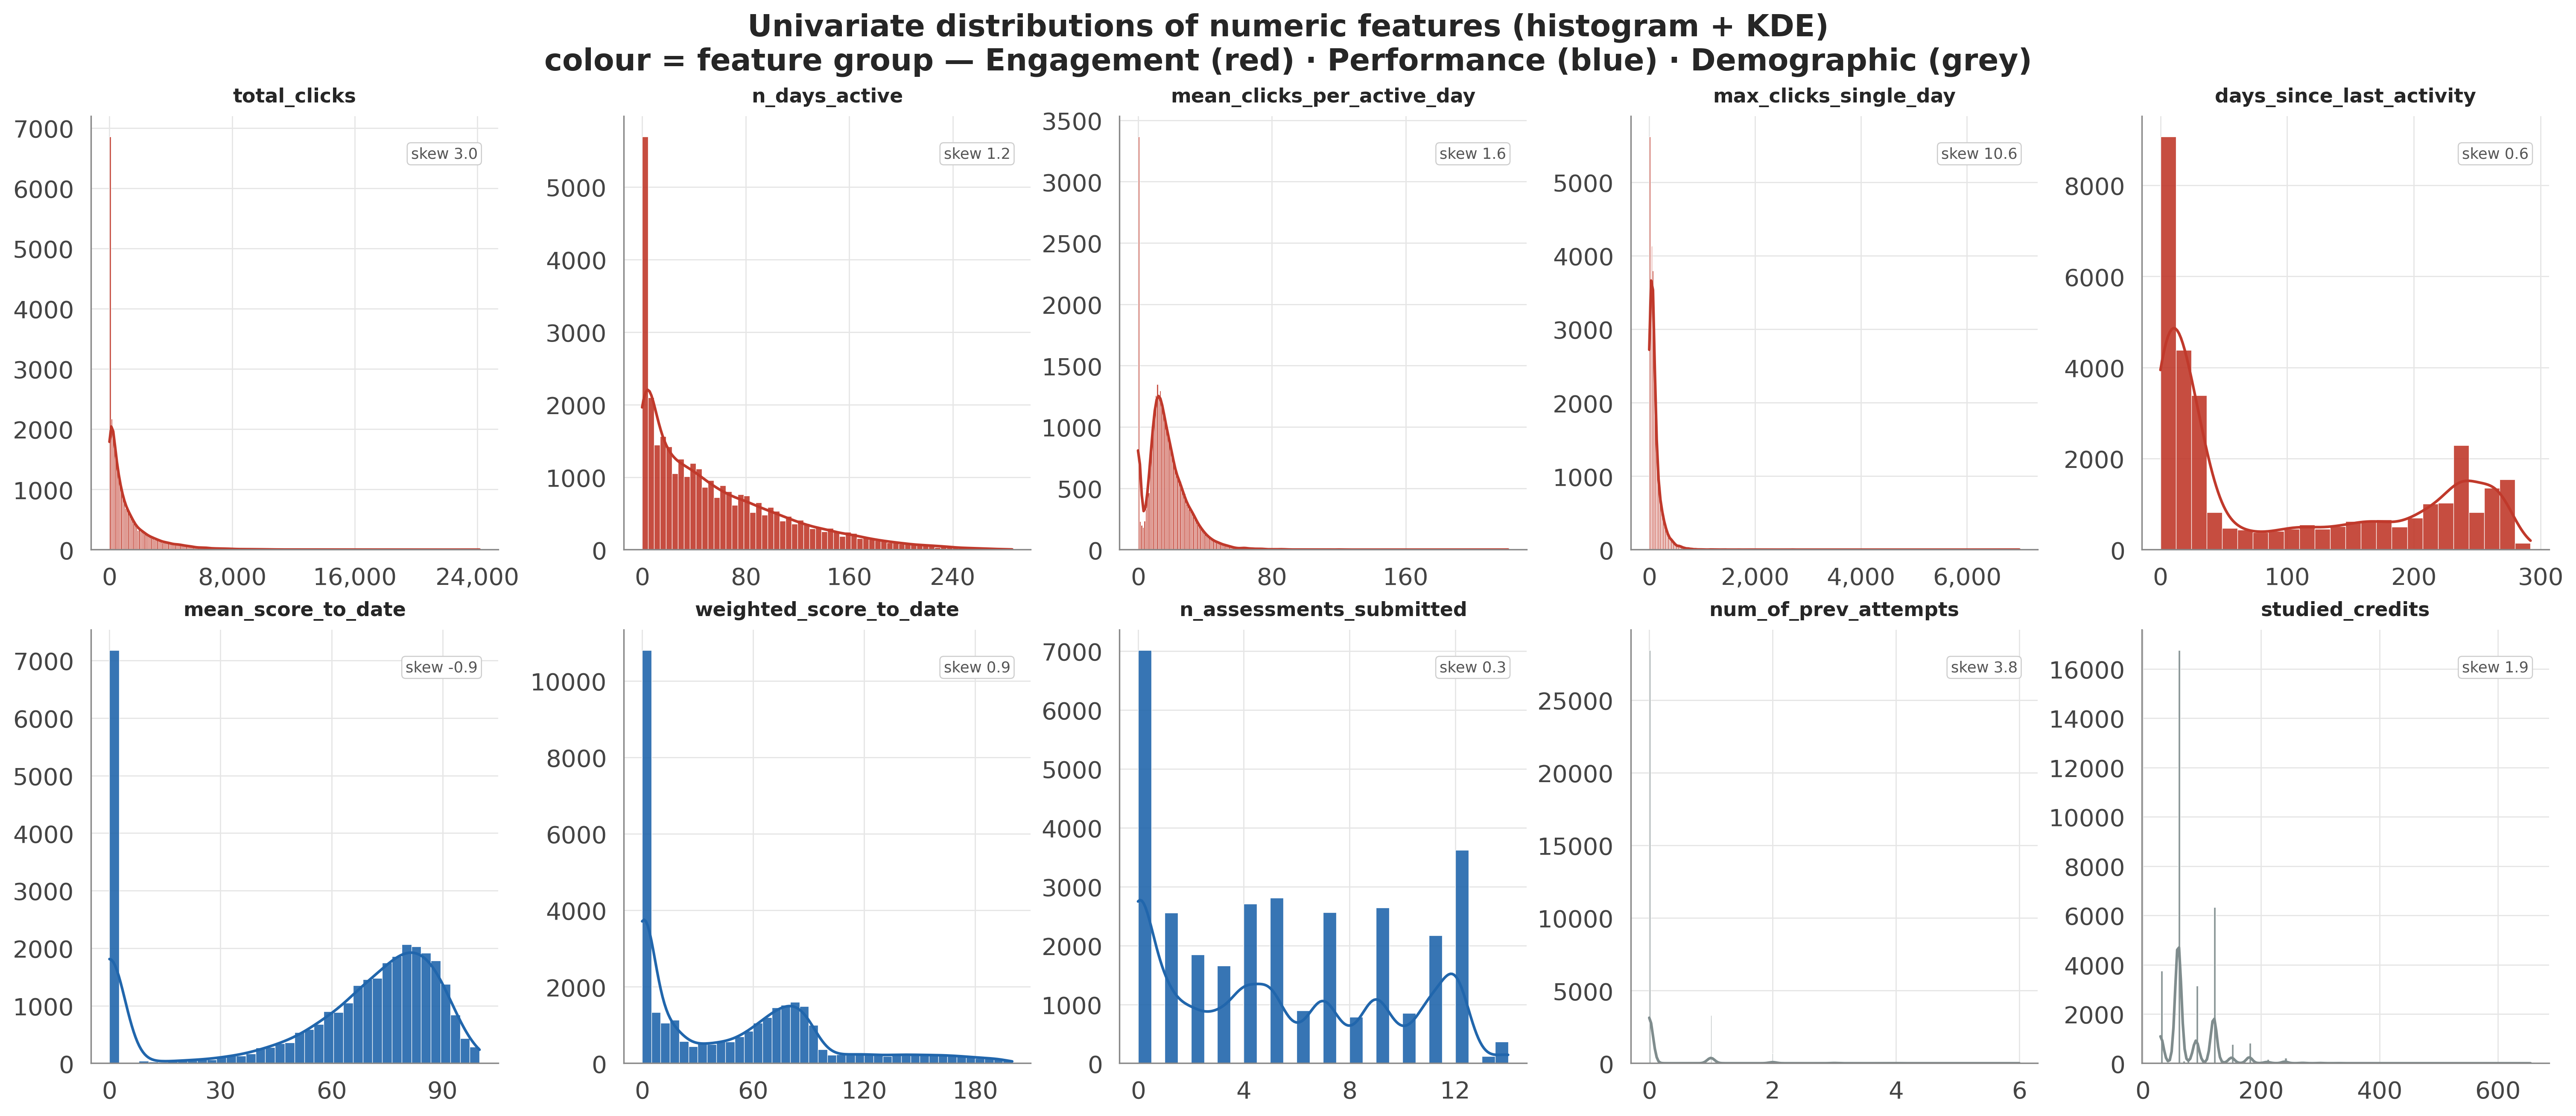
\includegraphics[width=\linewidth,height=0.74\textheight,keepaspectratio]{univariate_hist_kde.png}
    \end{column}
    \begin{column}{0.44\textwidth}
      \footnotesize\textbf{Histogram + KDE per numeric feature}
      \begin{itemize}\setlength\itemsep{0.3em}
        \item Most clickstream features are \textbf{strongly right-skewed}: \tcode{clicks\_resource} skew \textcolor{ccnured}{34.7}, kurtosis $\approx$2,125.
        \item Heavy tails are \textbf{real} outliers (super-active students) $\Rightarrow$ \tcode{log1p}, not deletion.
        \item \tcode{days\_since\_last\_activity} is \textbf{bimodal} — the disengagement signature.
        \item Non-normal $\Rightarrow$ non-parametric \textbf{Mann–Whitney} tests downstream.
      \end{itemize}
    \end{column}
  \end{columns}
\end{frame}

\begin{frame}{EDA — Numeric Features vs At-Risk (Cohen's $d$)}
  \begin{columns}[T]
    \begin{column}{0.52\textwidth}
      \centering
      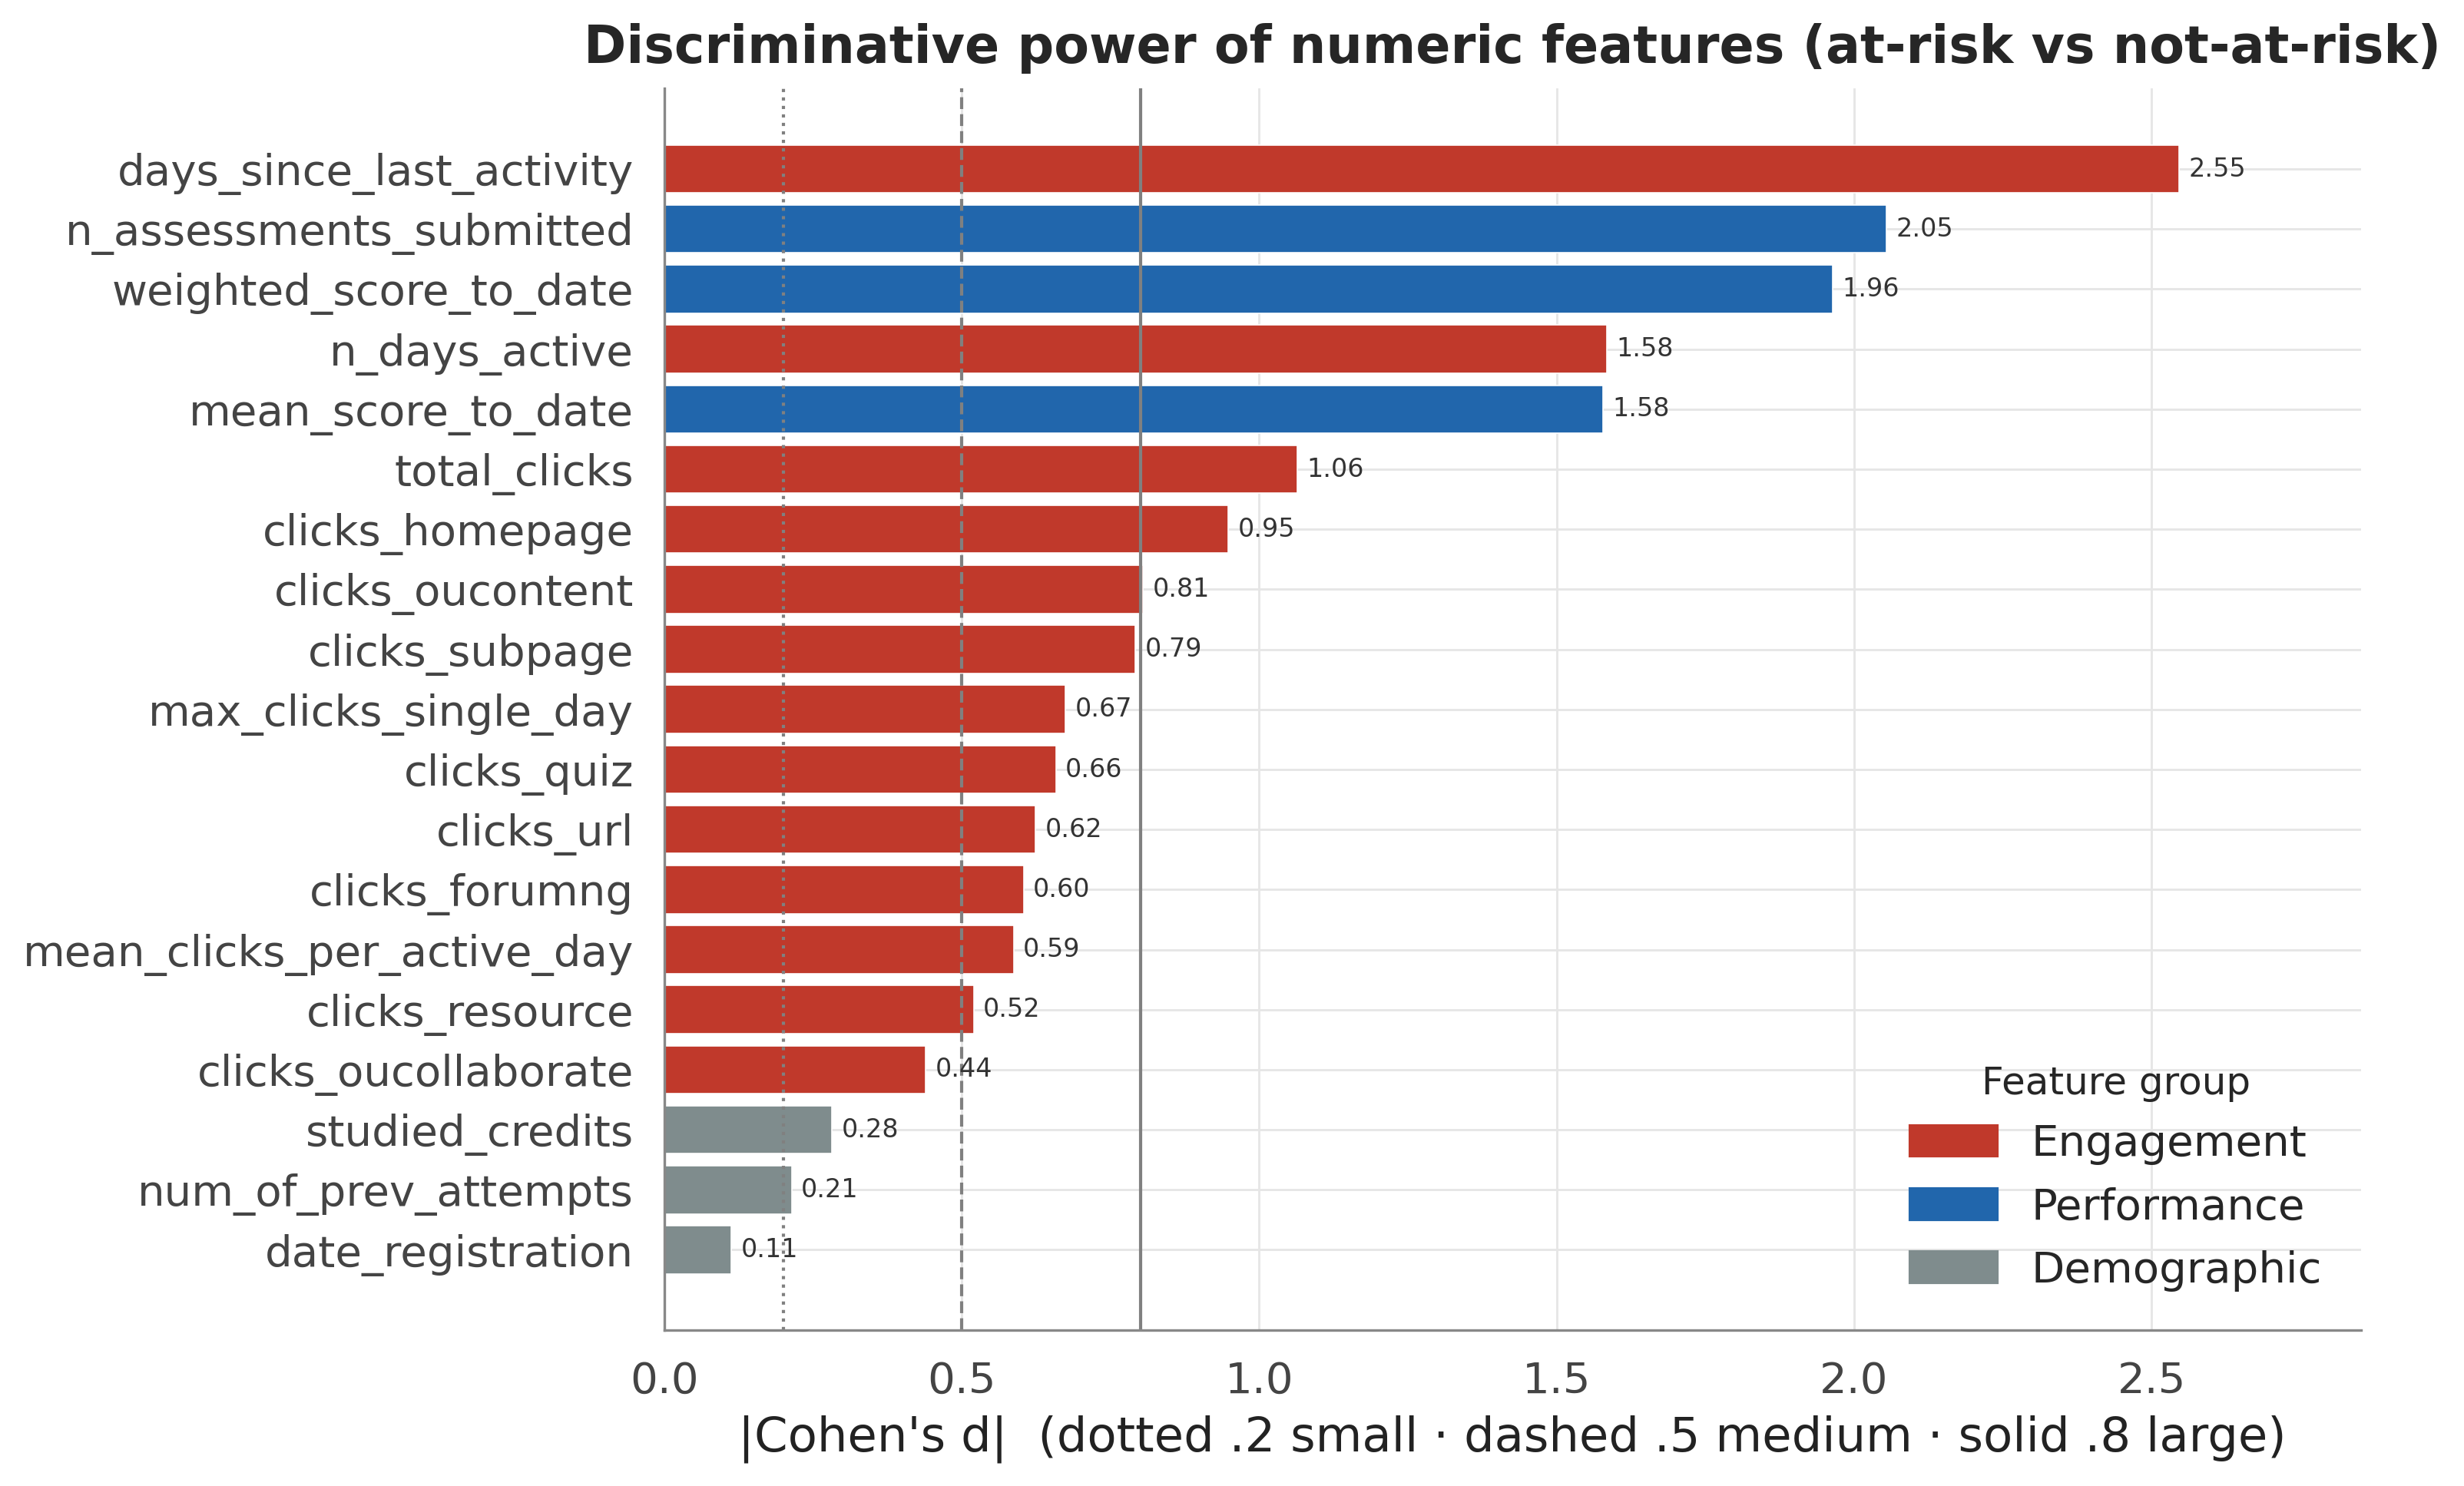
\includegraphics[width=\linewidth,height=0.76\textheight,keepaspectratio]{bivariate_effect_sizes.png}
    \end{column}
    \begin{column}{0.48\textwidth}
      \footnotesize\textbf{Effect size + Mann–Whitney (BH-corrected)}
      \begin{itemize}\setlength\itemsep{0.3em}
        \item Strongest: \tcode{days\_since\_last\_activity} \textcolor{ccnured}{$d=2.55$} (171 vs 14 days), \tcode{n\_assessments} 2.05 (2.3 vs 8.6), \tcode{weighted\_score} 1.96.
        \item \textbf{All 19/19} numeric features significant ($q<0.05$) — at n$\approx$32k, rank by \textbf{effect size}, not p.
      \end{itemize}
      \takeaway{Behaviour \& performance, not demographics, drive risk.}
    \end{column}
  \end{columns}
\end{frame}

\begin{frame}{EDA — Correlation \& Leakage Check}
  \begin{columns}[T]
    \begin{column}{0.52\textwidth}
      \centering
      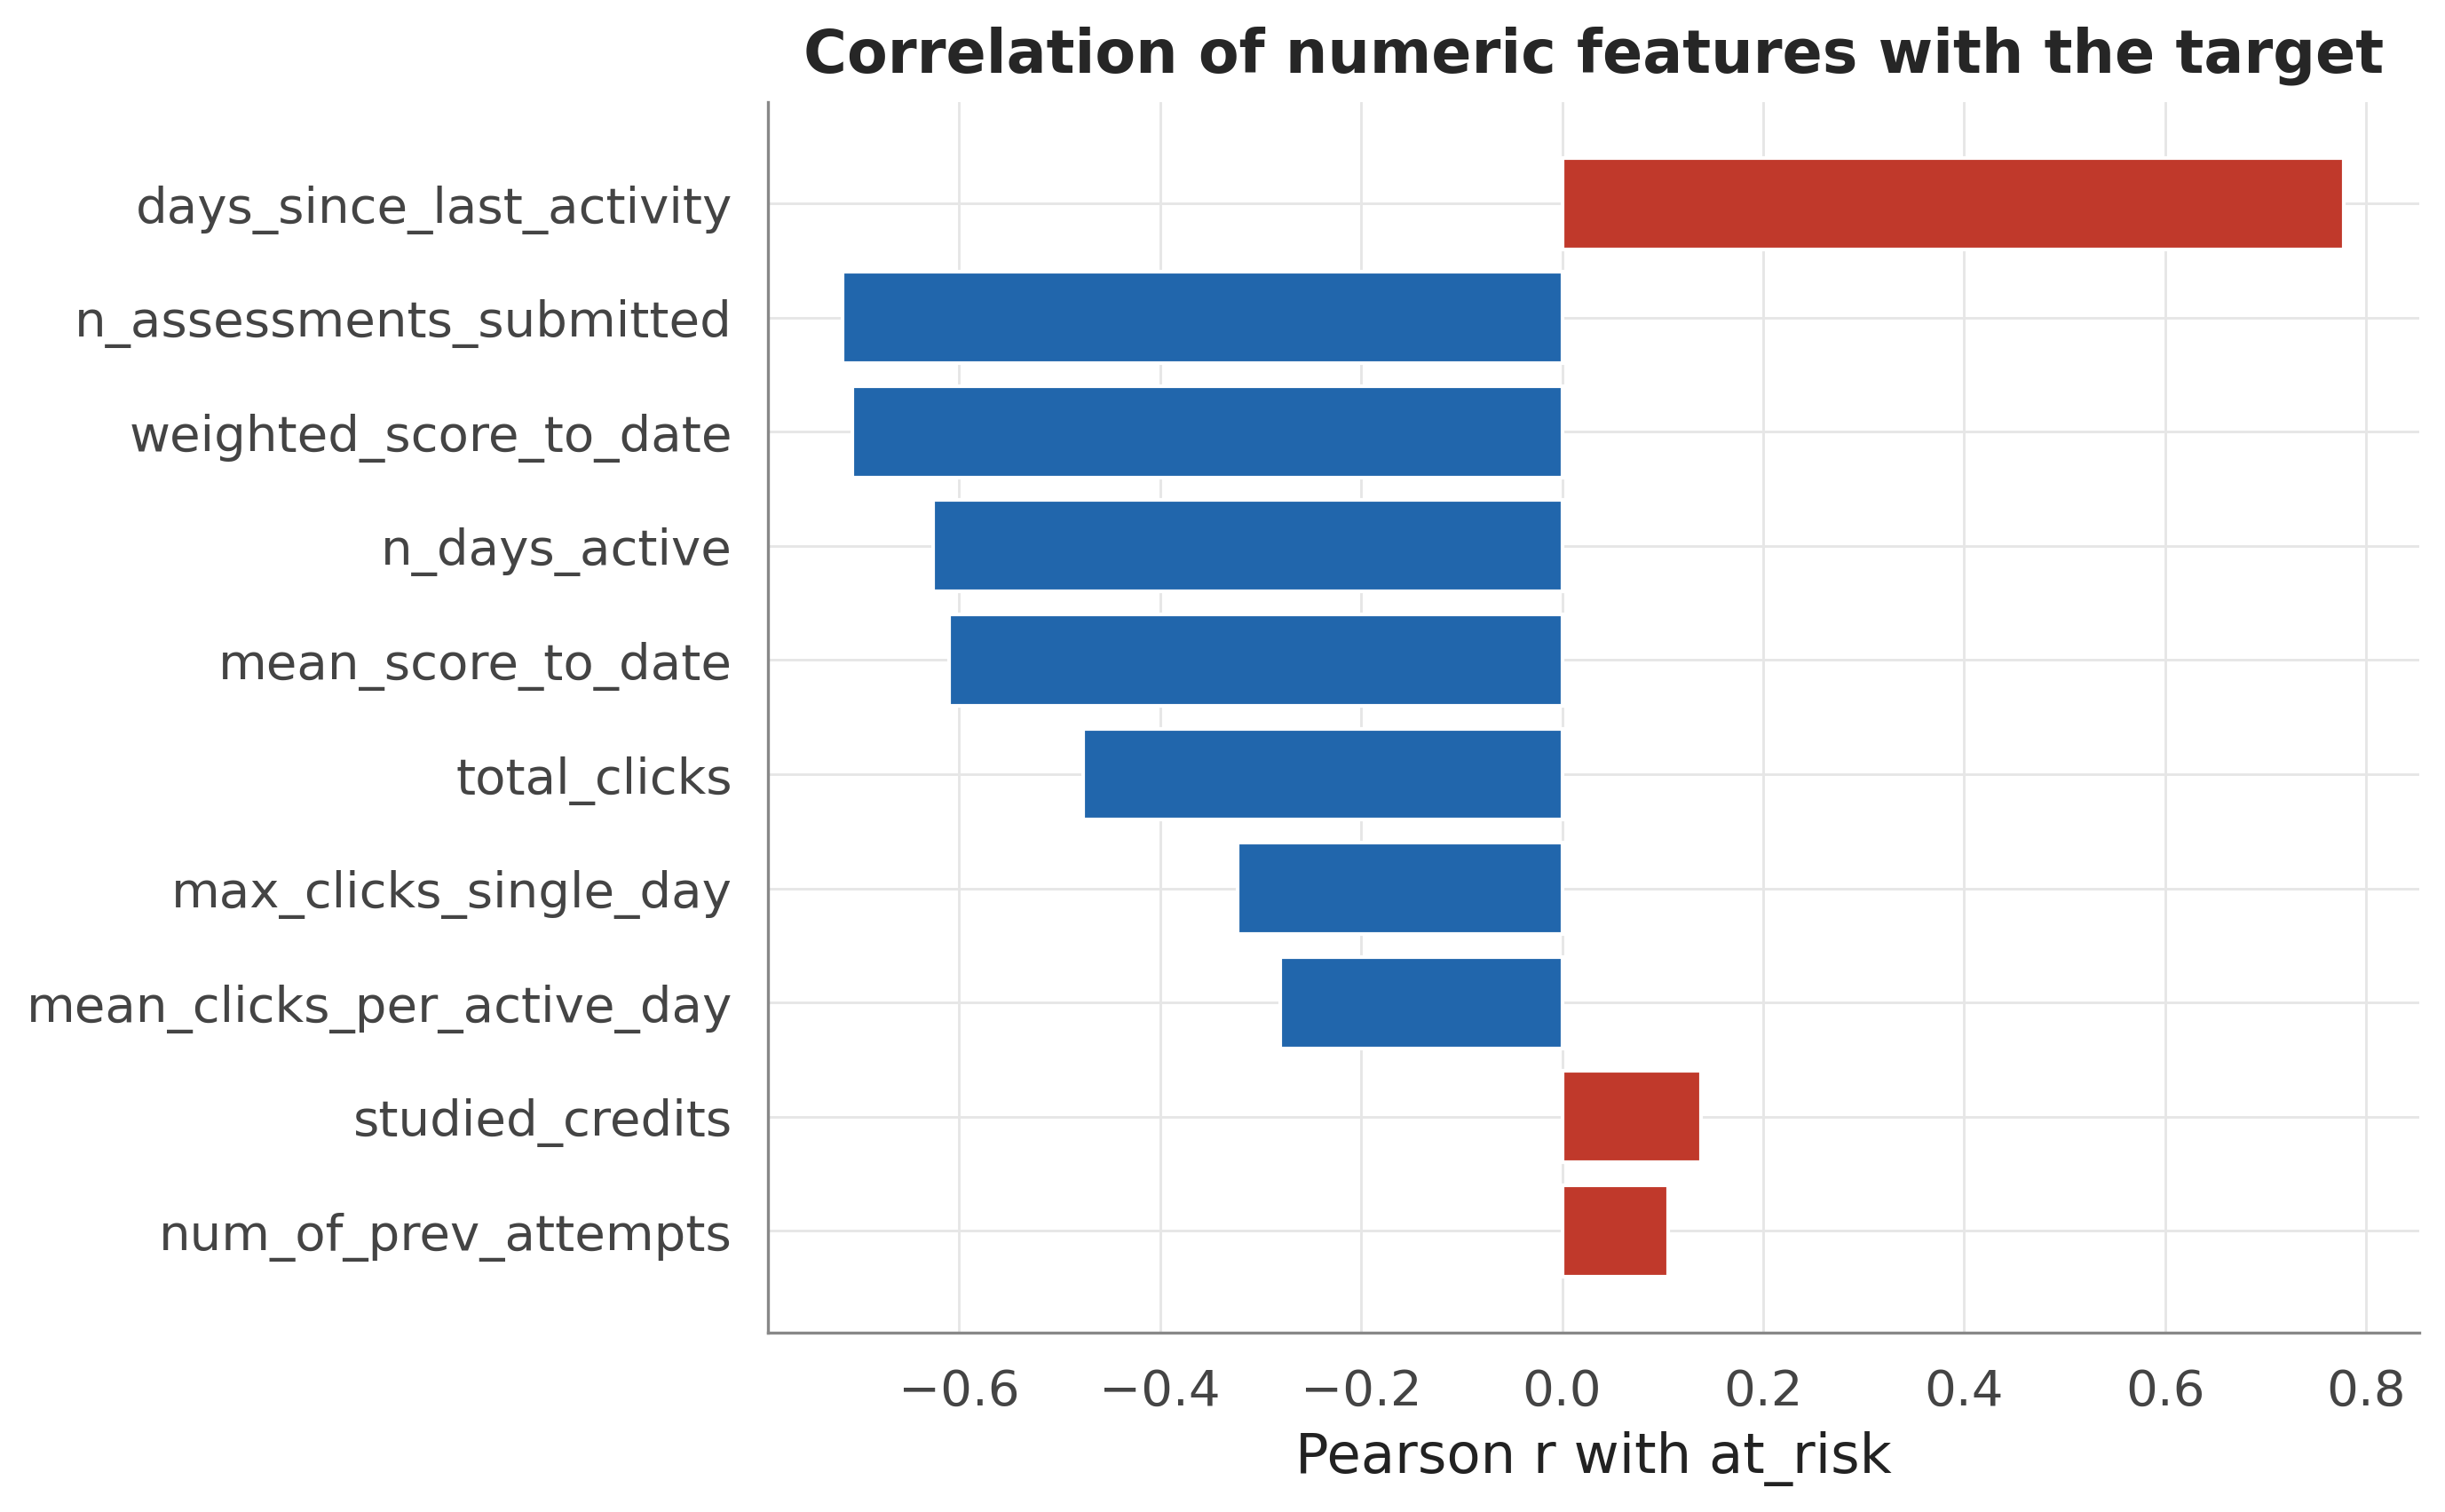
\includegraphics[width=\linewidth,height=0.76\textheight,keepaspectratio]{corr_with_target.png}
    \end{column}
    \begin{column}{0.48\textwidth}
      \footnotesize\textbf{Pearson + Spearman; correlation with the label}
      \begin{itemize}\setlength\itemsep{0.3em}
        \item Top $|r|$ with label: \tcode{days\_idle} \textcolor{ccnured}{+0.78}, \tcode{n\_assessments} $-$0.72, \tcode{weighted\_score} $-$0.71.
        \item 2 multicollinear pairs $|r|\geq0.8$ (\tcode{n\_days\_active}–\tcode{total\_clicks} 0.84) — flagged for SHAP.
        \item \textbf{No feature $|r|\geq0.95$} $\Rightarrow$ no leakage; demographic Cramér's V $\leq$ 0.15.
      \end{itemize}
      \takeaway{Independent methods (d \& r) agree $\Rightarrow$ trustworthy signal, no leakage.}
    \end{column}
  \end{columns}
\end{frame}

% =====================================================================
\section{Data Transformation \& Standardisation}
% =====================================================================
\begin{frame}{Variable Typing \& Encoding}
  {\footnotesize 28 input features $\to$ five types, each routed to the right transformer in one \tcode{ColumnTransformer}.}
  \vspace{3pt}
  {\footnotesize
  \setlength{\tabcolsep}{6pt}\renewcommand{\arraystretch}{1.3}
  \begin{tabularx}{\textwidth}{@{}l c Y >{\raggedright\arraybackslash}p{3.0cm}@{}}
    \toprule
    \rowcolor{ccnured}\hc{Type} & \hc{\#} & \hc{Examples} & \hc{Encoder / scaler}\\
    \midrule
    Numeric & 19 & clicks, scores, \tcode{studied\_credits} & \tcode{StandardScaler}\\
    \rowcolor{rowtint}Ordinal & 3 & \tcode{highest\_education}, \tcode{imd\_band}, \tcode{age\_band} & \tcode{OrdinalEncoder} (fixed order)\\
    Nominal & 3 & \tcode{region}, \tcode{code\_module}, \tcode{code\_presentation} & \tcode{OneHotEncoder}\\
    \rowcolor{rowtint}Binary & 2 & \tcode{gender}, \tcode{disability} & custom \tcode{BinaryEncoder}\\
    Indicator & 1 & \tcode{not\_submitted} & passthrough\\
    \bottomrule
  \end{tabularx}}
  \takeaway{Ordinal keeps the rank; one-hot avoids a false order; \tcode{drop=None} keeps every category visible for SHAP / LIME.}
\end{frame}

\begin{frame}{Standardisation: Before $\to$ After}
  {\footnotesize
  \setlength{\tabcolsep}{6pt}\renewcommand{\arraystretch}{1.35}
  \begin{tabularx}{\textwidth}{@{}>{\raggedright\arraybackslash}p{2.8cm} Y Y@{}}
    \toprule
    \rowcolor{ccnured}\hc{Component} & \hc{Before} & \hc{After}\\
    \midrule
    Labels & Dataset-specific class names & Binary: at-risk = 1, not = 0\\
    \rowcolor{rowtint}Categorical features & Text / category values & Encoded numeric (ordinal/one-hot/binary)\\
    Numeric features & Raw counts \& scores, skewed & \tcode{log1p}/winsorise + z-score scaled\\
    \rowcolor{rowtint}Feature matrix & 28 mixed-scale columns & \textbf{49}-column dense, 0 NaN\\
    Names & Raw column names & \tcode{snake\_case}, transformer-prefixed\\
    \bottomrule
  \end{tabularx}}
  \takeaway{\tcode{StandardScaler} (mean 0, sd 1) fitted on \textbf{train only}; applied to test with \tcode{.transform()} — never \tcode{.fit\_transform()}.}
\end{frame}

\begin{frame}{Preprocessing Sequence — Fit on Train Only}
  \begin{columns}[T]
    \begin{column}{0.52\textwidth}
      \centering
      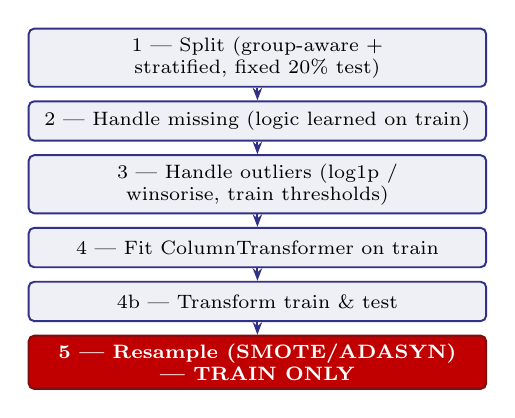
\begin{tikzpicture}[
        box/.style={draw=ccnunavy,line width=0.7pt,rounded corners=2pt,fill=ccnunavy!8,
          text width=5.6cm,align=center,font=\scriptsize,inner sep=3pt,minimum height=0.5cm},
        hl/.style={draw=ccnudark,line width=0.7pt,rounded corners=2pt,fill=ccnured,text=white,
          text width=5.6cm,align=center,font=\scriptsize\bfseries,inner sep=3pt,minimum height=0.5cm},
        arr/.style={-{Stealth[length=1.6mm]},ccnunavy,line width=0.7pt}]
        \node[box](a){1 — Split (group-aware + stratified, fixed 20\% test)};
        \node[box,below=0.16cm of a](b){2 — Handle missing (logic learned on train)};
        \node[box,below=0.16cm of b](c){3 — Handle outliers (log1p / winsorise, train thresholds)};
        \node[box,below=0.16cm of c](d){4 — Fit ColumnTransformer on train};
        \node[box,below=0.16cm of d](e){4b — Transform train \& test};
        \node[hl,below=0.16cm of e](f){5 — Resample (SMOTE/ADASYN) — TRAIN ONLY};
        \draw[arr](a)--(b);\draw[arr](b)--(c);\draw[arr](c)--(d);\draw[arr](d)--(e);\draw[arr](e)--(f);
      \end{tikzpicture}
    \end{column}
    \begin{column}{0.48\textwidth}
      \footnotesize\textbf{Why the order matters}
      \begin{itemize}\setlength\itemsep{0.3em}
        \item Split \textcolor{ccnured}{first} — nothing learned before the test set is set aside.
        \item Impute / encode / scale \textcolor{ccnured}{fit on train}, applied to test.
        \item Outlier thresholds per fold; \textcolor{ccnured}{no rows dropped}.
        \item Resample \textcolor{ccnured}{train only} — the test set keeps the real distribution.
        \item Mirrors the time-axis cut (\tcode{cut\_at\_checkpoint}).
      \end{itemize}
    \end{column}
  \end{columns}
\end{frame}

% =====================================================================
\section{Train/Test Split \& Leakage Control}
% =====================================================================
\begin{frame}{Split Design}
  {\footnotesize Three data properties constrain the split — so the design is grouped, stratified \emph{and} time-consistent.}
  \vspace{2pt}
  \begin{columns}[t,onlytextwidth]
    \begin{column}{0.32\textwidth}\begin{block}{1. Grouped}\scriptsize A student spans several module-presentations $\Rightarrow$ split by \tcode{id\_student} to avoid group leakage.\end{block}\end{column}
    \begin{column}{0.32\textwidth}\begin{block}{2. Imbalanced}\scriptsize At-risk $\approx$52.8\% $\Rightarrow$ \emph{stratify} so the test ratio cannot drift.\end{block}\end{column}
    \begin{column}{0.32\textwidth}\begin{block}{3. Time-aware}\scriptsize Six checkpoints share one axis $\Rightarrow$ the test set is \emph{identical} at every checkpoint.\end{block}\end{column}
  \end{columns}
  \vspace{4pt}
  {\footnotesize Design: 20\% hold-out (fixed once) + 5-fold $\times$ 5-seed CV via \tcode{StratifiedGroupKFold}. Verified on \tcode{master\_raw} (32,593 rows), identical across all 6 checkpoints:}
  \vspace{2pt}
  {\footnotesize
  \setlength{\tabcolsep}{7pt}\renewcommand{\arraystretch}{1.2}
  \begin{tabularx}{\textwidth}{@{}Y Y Y Y Y@{}}
    \rowcolor{ccnured}\hc{Train rows} & \hc{Test rows} & \hc{Test students} & \hc{At-risk (tr/te)} & \hc{Overlap}\\
    \midrule
    26,104 & 6,489 & 5,756 & .530 / .520 & \textbf{0}\\
    \bottomrule
  \end{tabularx}}
\end{frame}

\begin{frame}{Time-Aware Checkpoints}
  \begin{columns}[T]
    \begin{column}{0.42\textwidth}
      \footnotesize Features are recomputed at six course-progress checkpoints:
      \begin{center}\textcolor{ccnured}{\textbf{10 \textbullet{} 20 \textbullet{} 40 \textbullet{} 60 \textbullet{} 80 \textbullet{} 100\%}}\end{center}
      \begin{itemize}\setlength\itemsep{0.25em}
        \item Cutoff day = \tcode{round(length $\times$ t/100)}. e.g.\ AAA/2013J (268 d): t10=27, t40=107, t100=268.
        \item Only rows dated $\leq$ cutoff feed each checkpoint.
        \item Discrimination \textbf{grows with time} — early checkpoints are the hard, valuable ones.
      \end{itemize}
    \end{column}
    \begin{column}{0.58\textwidth}
      \centering
      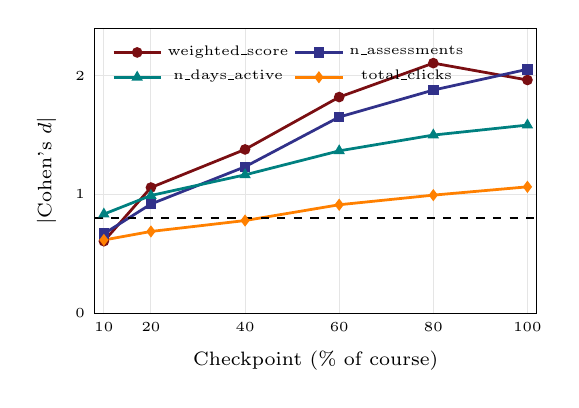
\begin{tikzpicture}
        \begin{axis}[width=7.2cm,height=5.2cm,
          xlabel={\scriptsize Checkpoint (\% of course)},ylabel={\scriptsize $|$Cohen's $d|$},
          xtick={10,20,40,60,80,100},xticklabel style={font=\tiny},yticklabel style={font=\tiny},
          ymin=0,ymax=2.4,xmin=8,xmax=102,
          legend style={font=\tiny,at={(0.02,0.98)},anchor=north west,draw=none,fill=none,legend columns=2},
          tick style={draw=none},grid=major,grid style={black!10},
          every axis plot/.append style={line width=1pt,mark size=1.4pt}]
          \addplot[ccnudark,mark=*] coordinates {(10,0.606)(20,1.058)(40,1.379)(60,1.820)(80,2.106)(100,1.964)};
          \addplot[ccnunavy,mark=square*] coordinates {(10,0.669)(20,0.919)(40,1.233)(60,1.652)(80,1.879)(100,2.054)};
          \addplot[teal,mark=triangle*] coordinates {(10,0.834)(20,0.991)(40,1.165)(60,1.367)(80,1.500)(100,1.584)};
          \addplot[orange,mark=diamond*] coordinates {(10,0.616)(20,0.688)(40,0.780)(60,0.913)(80,0.994)(100,1.064)};
          \addplot[black,dashed,line width=0.6pt,mark=none] coordinates {(8,0.8)(102,0.8)};
          \legend{weighted\_score,n\_assessments,n\_days\_active,total\_clicks}
        \end{axis}
      \end{tikzpicture}
    \end{column}
  \end{columns}
\end{frame}

\begin{frame}{Leakage Prevention — and It Is Tested}
  \footnotesize\textbf{Three temporal rules (per checkpoint $t$)}
  \begin{enumerate}\setlength\itemsep{0.2em}
    \item Drop assessment submissions with \tcode{date\_submitted > cutoff}.
    \item Drop VLE interactions with \tcode{date > cutoff} (via \tcode{cut\_at\_checkpoint}).
    \item Withdrawn-before-$t$ kept \& labelled at-risk — low activity is a legitimate early-warning signal, not leakage.
  \end{enumerate}
  \textbf{+ Fit-on-train principle:} every learner (imputers, encoders, scaler, resampler) is fit on the training fold only.
  \vspace{3pt}
  \begin{exampleblock}{Verified automatically by \tcode{tests/test\_leakage.py}}
    \centering{\large\bfseries 19 / 19 tests pass}\\[2pt]
    {\scriptsize no record beyond its cutoff \textbullet{} counts non-decreasing in $t$ \textbullet{} $t{=}100\%$ keeps all \textbullet{} 0 overlap \textbullet{} ratio preserved \textbullet{} train-only impute/winsorise \textbullet{} no-leak feature allow-list}
  \end{exampleblock}
\end{frame}

% =====================================================================
\section*{Summary}
% =====================================================================
\begin{frame}{Summary}
  \footnotesize
  \begin{enumerate}\setlength\itemsep{0.5em}
    \item[\textcolor{ccnured}{\textbf{01}}] \textbf{Required data} — OULAD supplies label, engagement, performance \& demographics at the \tcode{(student, module, presentation)} grain.
    \item[\textcolor{ccnured}{\textbf{02}}] \textbf{Collection} — a public, anonymised, CC-BY 4.0 benchmark used by the base studies $\Rightarrow$ reproducible \& comparable.
    \item[\textcolor{ccnured}{\textbf{03}}] \textbf{Cleaning} — duplicates, consistency, missing, outliers handled with no record dropped; parameters learned on train.
    \item[\textcolor{ccnured}{\textbf{04}}] \textbf{Transformation} — 28 features $\to$ typed encoders $\to$ a 49-column, leakage-safe, SHAP/LIME-ready matrix.
    \item[\textcolor{ccnured}{\textbf{05}}] \textbf{Split \& leakage} — fixed grouped/stratified 20\% test + 5$\times$5 CV; time-aware cuts; 19/19 tests pass.
  \end{enumerate}
\end{frame}

\begin{frame}[plain]{Thank you}
  \vfill\centering
  {\Huge\textcolor{ccnured}{Thank you}}\\[1.0em]
  {\footnotesize\textbf{Key references}}\\[0.3em]
  {\scriptsize
   Kuzilek, Hlosta, Zdrahal (2017), \emph{OULAD}, Scientific Data 4:170171 — CC-BY 4.0.\\
   Adnan et al.\ (2021), \emph{IEEE Access} 9.\quad Tomasevic et al.\ (2020), \emph{Computers \& Education} 143.\\
   Chawla et al.\ (2002), \emph{SMOTE}, JAIR.}
  \vfill
\end{frame}

\end{document}
